\documentclass{article}
\usepackage{gensymb, amsmath, float, graphicx, epstopdf}
\restylefloat{table}
\usepackage[margin=0.75in]{geometry}
\usepackage{multicol}
\begin{document}

\title{Lab Write-up 6: Impedance Matching and Frequency Tuning}
\author{Michael Shen}
\date{December 15, 2014}
\maketitle


\section{Testing the Matching Networks}

\subsection{Measured Data}
As measured in the previous lab and confirmed in this lab, $\omega_{0_{9cm}} = 46.973$ MHz.

\begin{enumerate}
	\item Measured output impedance for loop matching network \#1: 14.40 - j20.23 $\Omega$
	\item Measured output impedance for loop matching network \#2: 15.26 - j20.21 $\Omega$
	\item Measured output impedance for rectifier matching network: 2.312 - j30.54 $\Omega$
	\item Input return loss of matched rectifier: -21.904 dB
	\item Input return loss of matched system at 10cm: -26.527 dB
\end{enumerate}

\begin{table}[H]
\centering
\begin{tabular}{|c|c|}
\hline
Distance (cm) & Input Return Loss (dB) \\ \hline
2             & -0.702                 \\ \hline
4             & -1.880                 \\ \hline
6             & -5.117                 \\ \hline
8             & -10.631                \\ \hline
10            & -26.527                \\ \hline
12            & -10.627                \\ \hline
14            & -6.917                 \\ \hline
16            & -3.712                 \\ \hline
\end{tabular}
\end{table}

\subsection{Questions}

\begin{enumerate}
	\item A length of cable should not be used between the matching networks and the loops or the rectifier and its matching network because the cable will introduce an added electrical length because the system is not matched, very likely causing a phase shift and causing power to be reflected. It does not matter if there is a cable between the matched rectifier and the matched loops because these are already matched, so no power will be reflected.

\end{enumerate}


\section{Frequency-Tuned System}

\subsection{Measured Data}
\begin{table}[H]
\centering
\begin{tabular}{|c|c|c|}
\hline
Distance (cm) & Odd Mode Frequency (MHz) & Even Mode Frequency (MHz) \\ \hline
2             & 40.501                   & 63.172                    \\ \hline
4             & 43.372                   & 55.549                    \\ \hline
6             & 45.286                   & 53.008                    \\ \hline
8             & 46.474                   & 51.358                    \\ \hline
10            & 47.893                   & 49.672                    \\ \hline
12            & 48.817                   & 48.817                    \\ \hline
14            & 48.817                   & 48.817                    \\ \hline
16            & 48.817                   & 48.817                    \\ \hline
\end{tabular}
\end{table}

\begin{table}[H]
\centering
\begin{tabular}{|c|c|c|}
\hline
Distance (cm) & Constant Frequency $\vert S_{21}\vert$ (dB) 
& Frequency-Tuned $\vert S_{21}\vert$ (dB) \\ \hline
2             & -7.767                          & -0.621                       \\ \hline
4             & -4.622                          & -0.558                       \\ \hline
6             & -2.630                          & -0.663                       \\ \hline
8             & -1.176                          & -0.733                       \\ \hline
10            & -0.593                          & -0.743                       \\ \hline
12            & -0.938                          & -0.938                       \\ \hline
14            & -1.904                          & -1.904                       \\ \hline
16            & -3.360                          & -3.360                       \\ \hline
\end{tabular}
\end{table}

\subsection{Analysis}

\begin{enumerate}
	\item Using Eq. 6.33, $R_L = 14.83\Omega$, $\omega_0 = 46.974$ MHz, $R = 0.47\Omega$, and the mutual inductance values from the previous lab,
	\begin{table}[H]
	\centering
		\begin{tabular}{|c|c|c|}
		\hline
		Distance (cm) & M (nH)& $\eta_{\omega_0}$  \\ \hline
		2             & 822   & 0.4408  \\ \hline
		4             & 714   & 0.5358  \\ \hline
		6             & 492   & 0.7962  \\ \hline
		8             & 364   & 0.9280  \\ \hline
		10            & 278   & 0.9163  \\ \hline
		12            & 208   & 0.7733  \\ \hline
		14            & 174   & 0.6491  \\ \hline
		16            & 152   & 0.5519  \\ \hline
		\end{tabular}
	\end{table}

	\item Using Eq. 6.39, $\eta_{odd} = \dfrac{R_L^2}{(R+R_L)^2} = 0.9395$ for distances 2, 4, 6, 8, and 10 cm. Distances from 12-16 cm were not strongly coupled and did not have an odd mode frequency.
	\item Using Eq. 6.37, the maximum power transfer efficiency values are plotted below. \textbf{MATLAB CODE ATTACHED}
	\begin{figure}[H]
		\centering
   		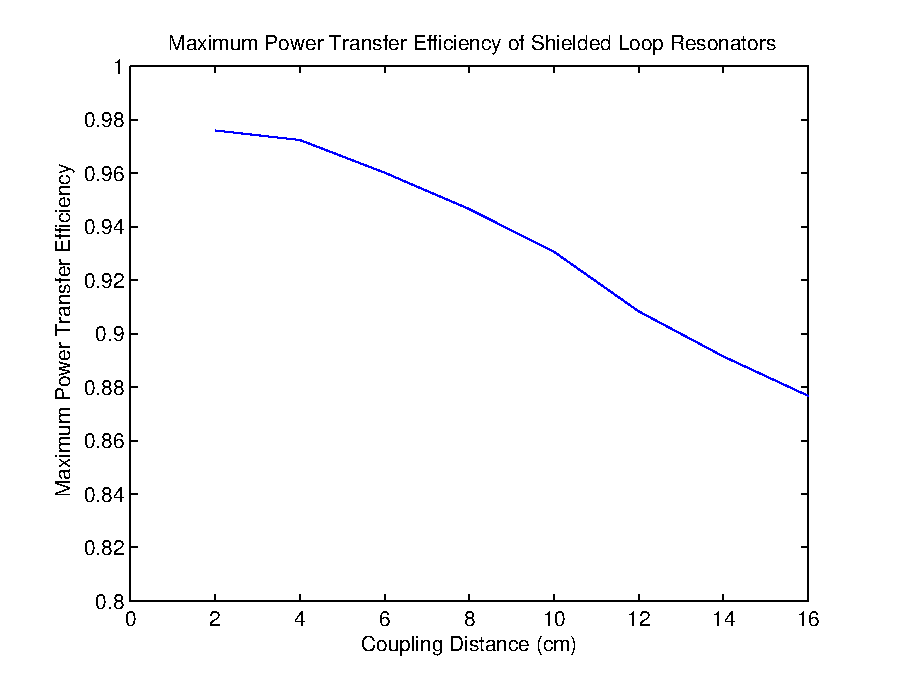
\includegraphics[scale = 0.85]{./Matlab/Analysis2_1.eps}
	\end{figure}
\end{enumerate}

\subsection{Questions}

\begin{enumerate}
	\item How does the input reflection coefficient of the matched system behave as the loops are moved away from the matching distance?
	\item Plot the theoretical efficiency and matched efficiency on the same axis, compare.
	\item Yes, the coupling distance of 10 cm has the minimum return loss and maximum $S_{21}$.
	\item Plot the theoretical efficiency vs measured efficiency for the frequency-tuned system, compare.
	\item Why is the critical coupling distance different.
\end{enumerate}

\section{Summary}
In this lab I learned the importance of frequency tuning, specifically that in strong coupling, odd and even mode frequencies result in less power loss than the resonant frequency. Furthermore, I learned how to design matching networks and rectifiers to allow sufficient power transfer to light up an LED.

\end{document}